\begin{abstract}
We study how a feature-learning model acquires \emph{skills} that are presented in context. Targets are additive models
$y=\sum_p c_p\,\sg(\langle v_p,x\rangle)$ with mean-zero task coefficients $c_p$, and a student with learned features and a
linear-in-label attention readout must recover the directions $v_p$ by online SGD from prompts of length $N$. For a single
skill of information exponent $k^*$ we obtain the population loss in closed form. As $N\to\infty$ it is the in-weight loss with the
link squared (effective exponent $2k^*$, a fact implicit in one-step analyses that we make dynamical). At finite $N$ the loss
acquires an \emph{alignment-dependent} variance term $\Gamma^2V(m)/N$, and the way the readout $\Gamma$ is parameterised decides what
this term does: a readout pinned at order one makes the unaligned state drift-stable below $m^*$, so that more prompts cannot
substitute for context length; a free scalar readout shrinks to a Wiener factor: for the population flow at fixed context length the exponent becomes $4k^*$ with escape time $\propto1/N$ (Theorem~B), while at accessible $d$ online SGD reproduces the flow's intermediate slowdown, set jointly by context length and the readout's initialisation and learning rate; a readout tied to the feature
norm removes the $N$-dependence as long as its initial norm is below an explicit threshold (proved, with the $N$-dependence bounded by $k^*\rho_0/(Nm_0^{2k^*-2})$). A parameter-free population ODE reproduces the exponents measured by online SGD at
$d=32$ for three readout protocols and four context lengths (all 12 cells within $0.5$ by a censored fit), the escape times at $d=64$ and $d=128$ including the predicted flip of a context length from escape to trap, and, at $k^*=3$, the trap threshold and an exponent near $6$ (two pre-registered precision bands were missed and are reported). With
many skills the dynamics decouple with emergence times $\propto1/\pi_p$; additive compositions of learned skills follow by linearity.
In small softmax transformers no parameter whose scale we froze reproduces the trap or the rescue (two pre-registered tests, both killed), and prompts per step partly substitute for context length, which the population loss cannot produce; the mechanism is open.
\end{abstract}
\section{Introduction}
\label{sec:intro}
Theories of feature learning explain \emph{when} a network acquires a direction $v$ in input space in terms of the information
exponent $k^*$ of the link function~\citep{benarous2021online}: online SGD needs $d^{k^*-1}$ samples ($d\log d$ for $k^*=2$). Large
models, however, acquire much of their behaviour as \emph{in-context} skills: the pretraining data presents a skill through
prompts whose labels are generated by a task-dependent coefficient, and the network must learn features that make the skill
recoverable from a context of length $N$. Recent analyses of in-context learning with learned features~\citep{oko2024pretrained,
nishikawa2025nonlinear,kim2024transformers,gu2026incontext} treat the context length as an \emph{inference-time} resource: it
controls how well a trained model estimates the task, and in one-step analyses of pretraining it enters only through
concentration, so that more prompts can substitute for longer prompts~\citep[Remark~3]{oko2024pretrained}.

We ask a different question: \emph{does the context length, together with how the readout is parameterised, change which
exponent governs the acquisition of a skill during pretraining?} We answer it in the smallest setting in which the question is
sharp---one or several skills with $k^*=2$ (even links, where in-weight learning is easy), a student with features on the sphere
and a linear-in-label readout, online SGD---and then test the predictions outside the solvable model.

\section{Setting}
\label{sec:setup}
Inputs $x\sim\mathcal N(0,I_d)$. A \emph{skill} is a unit vector $v_p\in S^{d-1}$ with link $\sg$; we use the normalised Hermite
polynomials $\sg_k=\mathrm{He}_k/\sqrt{k!}$, so $\E[\sg_j(\langle u,x\rangle)\sg_k(\langle w,x\rangle)]=\delta_{jk}\langle u,w\rangle^k$ for unit
$u,w$ and $k^*=k$. A \emph{task} is a coefficient vector $c$ with independent mean-zero entries, $\E c_p^2=s_p^2$; a \emph{prompt}
consists of $N$ pairs $(x_i,y_i)$ with $y=\sum_p c_p\sg(\langle v_p,x\rangle)$ and a query $(x_q,y_q)$ from the same task. With a
dictionary of $P$ skills and single-skill prompts, skill $p$ appears with frequency $\pi_p$.

\paragraph{Model A (in-context).} Features $\phi_j(x)=\sg(\langle w_j,x\rangle)$, $w_j\in S^{d-1}$, and a linear-in-label readout
\begin{equation}
\hat y_q=\sum_j\Gamma_j\,\phi_j(x_q)\,A_j,\qquad A_j=\frac1N\sum_{i=1}^N y_i\,\phi_j(x_i),
\label{eq:modelA}
\end{equation}
the MLP-plus-linear-attention architecture of \citet{oko2024pretrained}. We consider three readout protocols: \emph{fixed}
$\Gamma_j=\gamma$; \emph{free}, a trainable scalar; and \emph{tied}, $\Gamma_j=\|u_j\|^2$ with $w_j=u_j/\|u_j\|$ (the 2-homogeneous
student of \citet{ren2025emergence}). \textbf{Model B (in-weight)} is ordinary regression $\hat y=\sum_j a_j\phi_j(x)$ on the fixed
task $c\equiv a$. Both are trained by online spherical SGD on the square loss with fresh data at every step: $B$ prompts per step, step size
$\eta$ on the features, step size $\eta_\Gamma$ on a free readout initialised at $\Gamma_0$,
and for the tied readout an unnormalised $u$ with $\|u_0\|^2=\rho_0$. We report escape times $T_{0.5}$ (steps until $|m|\ge\tfrac12$) and
their \emph{flow-time} version $T_{0.5}\,\eta$, which is what the population ODEs predict; the single-feature experiments initialise
at $m_0=c\,d^{-1/2}$ exactly.

Write $g(m)=\sum_k\alpha_k^2m^k$ for $\sg=\sum_k\alpha_k\sg_k$ and $V(m)=\E[\sg(\langle v,x\rangle)^2\sg(\langle w,x\rangle)^2]=\sum_j\beta_j^2m^j$
where $\sg^2=\sum_j\beta_j\sg_j$. For $\sg_2$: $g=m^2$, $V=1+8m^2+6m^4$.

\section{A single skill}
\label{sec:single}

\begin{proposition}[Population loss]
\label{prop:loss}
For $P=1$, one feature at overlap $m=\langle w,v\rangle$, readout $\Gamma$ and $\E c^2=s^2$,
\begin{equation}
\begin{aligned}
L_A(m)&=s^2\Big[1-2\Gamma g(m)^2+\Gamma^2 g(1)\Big((1-\tfrac1N)g(m)^2+\tfrac{V(m)}{N}\Big)\Big],\\
L_B(m)&=1-2a\,g(m)+a^2g(1).
\end{aligned}
\label{eq:LA}
\end{equation}
\end{proposition}
(Proof: Appendix.)

\paragraph{The link is squared.} As $N\to\infty$, $L_A=s^2[1-2\Gamma g^2+\Gamma^2g(1)g^2]$ depends on $m$ only through $g(m)^2$, whereas
$L_B$ depends on it through $g(m)$. Near $m=0$ the drift is $2\Gamma s^2(2-\Gamma g(1))\,k^*\alpha_{k^*}^4m^{2k^*-1}$ against
$2ak^*\alpha_{k^*}^2m^{k^*-1}$ for Model B.

\begin{proposition}[Finite context: a drift-stable unaligned state]
\label{prop:repulsion}
For $\sg_2$ and fixed readout $\Gamma=\gamma$, $-\partial_mL_A=s^2\big[(8\gamma-4\gamma^2(1-\tfrac1N)-24\gamma^2/N)m^3-16\gamma^2m/N\big]$. For
$\gamma<\gamma_1=2N/(N+9)$ the origin is a local minimum of $L_A$, the drift is repulsive for $m<m^*$ and attractive on $(m^*,1)$, with
$m^{*2}=4\gamma/\big(2N-(N+5)\gamma\big)\approx2\gamma/(N(1-\gamma/2))$ (for $\gamma\ge\gamma_1$ the overlap decays from every $m_0<1$).
\end{proposition}
A feature initialised at $m_0\approx d^{-1/2}$ is attracted
only if $d\lesssim d^*=N(8-4\gamma(1-\tfrac1N)-24\gamma/N)/(16\gamma)$ ($\approx31$ for $\gamma=1$, $N=128$).

\begin{proposition}[Readout parameterisation: three regimes---informal summary of Theorems~\ref{thm:A}--\ref{thm:B} and Prop.~\ref{prop:joint}, Appendix~\ref{app:thm}]
\label{prop:shrink}
Consider the population gradient flow of~\eqref{eq:LA} for $\sg=\sg_2$ in flow time $t=\eta\cdot\text{steps}$, started at $m_0=d^{-1/2}$,
and let $\tau_{\rm esc}$ be the time to reach $m=\tfrac12$.
\begin{enumerate}
\item[(a)] \emph{Pinned readout} $\Gamma=\gamma$.
If $m_0<m^*(\gamma,N)$ then $\tau_{\rm esc}=\infty$; otherwise $\tau_{\rm esc}=\Theta(m_0^{-2})$ for $m_0$ bounded away from $m^*$, diverging logarithmically as $m_0\downarrow m^*$ (Theorem~\ref{thm:A}(ii)), with an $N$-dependence that saturates for $N\gg\gamma d$.
The condition involves $N$ and $\gamma$ only---not the number of prompts per step, which does not enter the population drift.
\item[(b)] \emph{Free scalar readout} $\dot\Gamma=-r\,\partial_\Gamma L_A$, $r=\eta_\Gamma/\eta$, $\Gamma(0)=\Gamma_0$. The fixed point of $\Gamma$ at given $m$ is
$\Gamma^*(m)=g^2/\big(g(1)[(1-\tfrac1N)g^2+V/N]\big)$, approached at rate $2r\,g(1)[(1-\tfrac1N)g^2+V/N]\approx2r/N$. \emph{Adiabatic case}
($2r/N\gg$ the overlap rate): the overlap sees $L_A(m,\Gamma^*)$, whose exponent is $4k^*$ for $m^{2k^*}\ll V/N$ and $2k^*$ otherwise, and in the
former regime $\tau_{\rm esc}\propto m_0^{-(4k^*-2)}/N$ (Appendix~\ref{app:deriv}). \emph{Growth-limited case} ($2r/N\lesssim$ the overlap rate; E2 at $N=16$ is adiabatic to $1\%$, the other cells are not): $\Gamma$ lags $\Gamma^*$ and $\tau_{\rm esc}$ depends on $(N,\Gamma_0,r)$ jointly; the ODE gives intermediate
$N$-dependences (e.g.\ $\tau(16)/\tau(256)=4.4$ at $d=64$, $\Gamma_0=0.01$, $r=1$, against $16$ in the adiabatic $1/N$ law).
\item[(c)] \emph{Tied readout} $\Gamma=\rho=\|u\|^2$, features $\sg(\langle u/\|u\|,x\rangle)$. The directional velocity is
$(1-m^2)\big[4gg'-\rho\,(2(1-\tfrac1N)gg'+V'/N)\big]$, which is exactly the pinned velocity at $\gamma=\rho$ divided by $\rho$ (norm-independence
of the attraction, \citealp[Lemma~B.1]{ren2025emergence}): a tied readout behaves like a pinned readout of value $\rho(t)$ under a time
change. From a small $\rho_0$, $\dot\rho=-4\rho\,\partial_\rho L_A$ leaves $\rho$ near $\rho_0$ and $\tau_{\rm esc}=\Theta(m_0^{-2})$ is independent of
$N$ provided $\rho_0\le\rho^*(m_0)/4$ (Theorem~\ref{thm:A}(iii)(c): $\rho(t)$ then stays within explicit factors of $\rho_0$ and $\big|\tau_{\rm esc}(2k^*-2)4k^*m_0^{2k^*-2}-1\big|\le C_k\big(k^*\rho_0/(Nm_0^{2k^*-2})+\rho_0+\lambda_km_0^2\big)$, $C_2=C_3=4$; the qualifier was added after E6, and the two cells where $N$-dependence appeared---E5's $\rho_0=0.1$, $N=16$ and E6's $N=16$, $d=16$---are exactly those violating the hypothesis)---within it the tied readout self-selects the small-readout regime. Let $\rho^*(m)=2Nm^2/\big(4+(N+5)m^2\big)\approx Nm^2/2$ be the value at which the
directional drift vanishes. For $\rho_0>\rho_{\rm trap}(m_0)$ (Theorem~\ref{thm:A}(iii); $\rho_{\rm trap}\to c_2\rho^*$ with $c_2=\tfrac43$ as $m_0\to0$, Remark~\ref{rem:ck}; at $d=64$, $N=16$, $\rho_{\rm trap}=0.178$ against $c_2\rho^*=0.154$; between $\rho^*$ and $\rho_{\rm trap}$ the overlap first
falls and then escapes, proved for the small-$m$ system), the population flow traps permanently ($m\propto t^{-2}$ while $\rho\propto t^{-1}$, so $\rho$ never falls below the
moving threshold); under SGD,
noise keeps $m$ at the noise floor while $\rho$ decays, and the feature is eventually released---a long delay rather than a trap (E5).
\end{enumerate}
\end{proposition}
That a fast readout doubles the exponent of an in-weight problem is
known~\citep[\S5]{bietti2023learning}; what is specific to the in-context problem is that the finite-context noise drives the
readout towards $\Gamma^*$, so that \emph{whether context length trades off against training time, is irrelevant, or is a
hard requirement is decided by how the readout is parameterised}.

\paragraph{E1: exponents by SGD.}
Here ($d=32$) the slope of $\log T_{0.5}$ against $\log m_0$ estimates $\kappa_{\rm eff}=2-\text{slope}$. Fig.~\ref{fig:kappa} (Appendix) shows $\kappa_{\rm eff}$ for free
($\eta_\Gamma=\eta$ and $10\eta$) and tied readouts at $N\in\{32,128,512,4096\}$ against the population ODE of
Props.~\ref{prop:loss}--\ref{prop:shrink} evaluated \emph{after the run} at the same $d$, $m_0$-grid, $\Gamma_0$ and $\eta_\Gamma/\eta$ (the ODE
itself was fixed before the run; its evaluation at these parameters was not pre-registered): tied $4.10$--$4.44$ (ODE $4.15$--$4.18$); free
$4.8$--$6.6$ rising as $N$ falls (ODE $4.85$--$7.0$).
With a censored (Tobit) fit for the three cells that contain censored runs, all twelve cells agree with the ODE within $0.5$
the estimator is a
secant over a factor $2.8$ in $m_0$ and local slopes vary, so these are effective, not asymptotic, exponents.
Two pre-registered predictions in this experiment failed and are
reported as such: the learned $\Gamma$ at $T_{0.5}$ is $0.18$--$0.25$, below $\Gamma^*(0.5;N)=0.38$--$0.99$, and a scan of $T_{0.5}$ against $d\le48$ at $N=128$ versus $2048$ showed
no $N$-dependence, which is what the ODE predicts for $d\le48$ but means the $N$-dependence is
established only through $\kappa_{\rm eff}(N)$ at fixed $d$.

\paragraph{E2 and E7: the three regimes by SGD (Exps.~6 and 10, pre-registered P23).}
To test Prop.~\ref{prop:shrink} directly (Fig.~\ref{fig:regimes}) we fix $d=64$, $m_0=d^{-1/2}$, $\eta=1/d^2$, vary $N\in\{16,64,256\}$ under two schemes---tokens per
step fixed ($NB=4096$) and prompts per step fixed ($B=64$)---and run the four protocols, three seeds each, with the population
escape times computed before the run. Pinned $\gamma=1$: no escape at $N\le64$ in $10^6$ steps ($0/9$), $3/6$ at $N=256$
($d^*\approx63$); pinned $\gamma=0.1$: median $396$k$/192$k$/179$k steps against $400$k$/193$k$/175$k predicted; free: $1.78$M$/614$k$/402$k
against $1.82$M$/623$k$/409$k, ratio $T(16)/T(256)=4.4$ as predicted ($4.44$)---the growth-limited value of
Prop.~\ref{prop:shrink}(b), not the adiabatic $1/N$ law; tied: $17.0$k$/15.1$k$/14.0$k against $17.0$k$/16.4$k$/16.3$k.
Repeating E2's protocols at $d=128$ ($\eta=1/d^2$, three seeds): the pinned $\gamma=0.1$ cell at $N=16$, which escaped at $d=64$, is now censored
$3/3$ at $2.5\cdot10^6$ steps---the flip across $d^*(16)=76$ of Prop.~\ref{prop:shrink}(a)---while $N=64,256$ escape at $0.99$ and $1.01$ of the flow
time ($N$-saturating); the tied readout stays
$N$-flat (medians/flow $1.12,0.97,1.02$; $T(16)/T(256)=1.20$, flow $1.09$); the free readout at $N=256$ takes $5.29\cdot10^6$ steps ($0.985$ of the
flow) and its secant exponent across $d=64\to128$ is $5.4$ (flow $5.4$), between the signal-dominated $4$ and the adiabatic $8$.

\begin{figure*}[t]
\centering
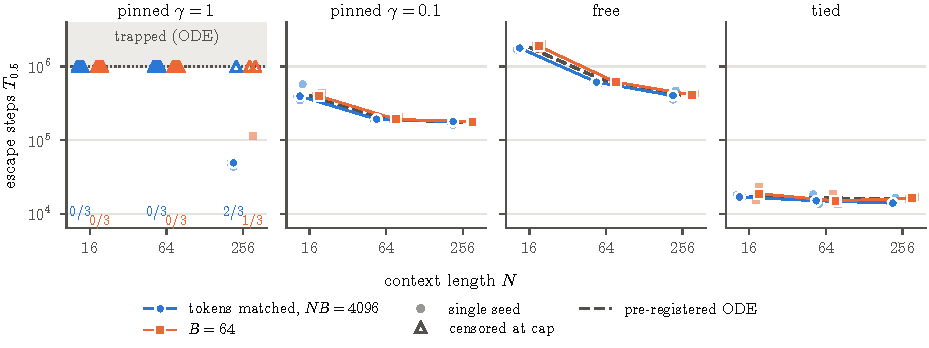
\includegraphics[width=.62\textwidth]{figs/fig_regimes.pdf}
\caption{Escape steps $T_{0.5}$ against context length $N$ for the four readout protocols ($d=64$, $\eta=1/d^2$,
$m_0=d^{-1/2}$). Light markers are single seeds (three per cell), solid markers and lines the median over seeds, for
tokens per step fixed ($NB=4096$, circles) and prompts per step fixed ($B=64$, squares). Open triangles are runs that had not escaped at the
step cap ($10^6$) and are drawn at the cap; the counts under the pinned-$\gamma=1$ panel are runs escaped out of $3$. Dashed lines are the
population-ODE escape times (flow time $\times d^2$), \emph{fixed before the run}.}
\label{fig:regimes}
\end{figure*}

\paragraph{E5: controls.}
Varying the readout's initial value and learning rate (free: $\Gamma_0=0.1$ or $\eta_\Gamma=10\eta$ at $d=64$) changes the $N$-ratio from $4.4$ to
$9.2$ and $10.7$ (ODE $9.1$ and $8.9$; medians within $2\%$ except the $\eta_\Gamma=10\eta$, $N=16$ cell, $24\%$ slow), confirming that the
free-readout exponent is a function of $(N,\Gamma_0,\eta_\Gamma/\eta)$, as Prop.~\ref{prop:shrink}(b) states. A tied readout started at $\rho_0=0.3>\rho_{\rm trap}(m_0)=0.18$ at $N=16$ was pre-registered to trap (the deterministic flow provably does, Theorem~\ref{thm:A}(iii)); under SGD all three seeds escaped after a $\approx30\times$ delay, once $\rho$ had
decayed to $0.012$---so under SGD tying converts the pinned trap into a delay, and the pre-registered wording "the repulsion survives tying" is
withdrawn in favour of "is delayed by tying". Finally, scaling the step size with the batch ($\eta\propto B$, pinned $\gamma=0.1$, $N=64$)
leaves the escape \emph{flow time} invariant to $0.5\%$ while steps scale as $1/\eta$: the irrelevance of prompts per step in E2 is a
statement about flow time, independent of how $\eta$ is chosen.

\paragraph{E6: a $k^*=3$ check (Exp.~9, pre-registered P22).}
With $\sg=\sg_3$, $\eta=2\cdot10^{-4}$, $B=64$, $d\in\{8,16,32\}$, three seeds: the tied readout ($\rho_0=0.01$, $N=128$)
gives medians $1.18/0.89/0.80$ of the flow ($d=8/16/32$; the pre-registered band was $15\%$, so P22a failed) and secant exponents $5.7$ and $6.0$ (ODE $6.5$, $6.4$; the $8\to16$ secant misses its $\pm0.5$ band)---an exponent near $6$, against $\approx4$ at $k^*=2$. Two post-hoc controls, declared before running: at $\eta/4$ the $d=8$ ratio becomes $1.007$ (discretisation); at $B=256$ the $d=32$ ratio becomes $1.14$, outside the $10\%$ band we had declared for it, so the flow is confirmed only to $\approx15\%$ there.
The pre-registered $N$-flatness of the tied readout (P22b) \emph{failed} at $N=16$, $d=16$: the flow predicts $1.6\times$ the $N=128$ time,
the seeds gave $47$k, $500$k and censored, and at $d=32$ all three seeds trapped (predicted: $\rho_0=0.01>\rho_{\rm trap}=0.006$); the statement that survives is the conditional one in
Prop.~\ref{prop:shrink}(c): $N$-flat for $\rho_0\ll\rho_{\rm trap}(m_0,N)$.

\section{Many skills and composition}
\label{sec:many}
\textbf{E3} ($d=32$, $P=16$, $\pi_p\propto p^{-1.5}$, $M=64$, fixed $\Gamma=0.1$, three seeds) gives slopes of $\log T_p$ versus $\log p$ of
$1.44\pm0.08$ for the in-context model, against $0.75\pm0.08$ for a capacity-matched in-weight baseline and $0.75$--$0.89$ for the
2-homogeneous in-weight student of \citet{ren2025emergence} (Appendix).

\section{Transformers: an observation and what it excludes}
\label{sec:transformer}
We train two-layer softmax transformers (4 heads, pre-LN, Adam, online data; Fig.~\ref{fig:transformer}, Appendix) on the same in-context task with $k^*=2$.
\textbf{Large initial alignment} ($d=32$, MLP width 256): at a fixed
$8192$ tokens per step the emergence step \emph{increases} with $N$ ($1000/1400/2800$ for $N=16/64/256$)---fewer prompts per step dominate. \textbf{Small initial alignment} ($d=256$, width 32): $N=16$ with $B=64$ prompts never emerges in $30$k steps
($3/3$); $N=16$ with $B=1024$ (the tokens per step of $N=256$, $B=64$) emerges in all three seeds ($10.6$--$14.8$k), $\approx3\times$ later than $N=256$ in two
paired seeds ($2.8$--$4.0$k) and earlier in the third ($11.6$k against a run censored at $17$k). Neither pre-registered extreme (a trap; interchangeability)
held. These are observations, not a test of Sec.~\ref{sec:single}: the Adam step was not rescaled with $B$ (Appendix).

\paragraph{Two null knob tests (Exps.~8 and 11; pre-registered P21, P24).}
If Prop.~\ref{prop:shrink} acted through a scalar readout, freezing the final head, or the attention output projections of both blocks, at their O(1)
initial norm should trap $N=16$ even at $B=1024$, and freezing them at $0.1\times$ should rescue $N=16$, $B=64$. Neither happened for either knob (two
seeds per cell; both kill criteria met): $B=1024$ rescued $N=16$ under every frozen protocol that ran ($5.8$k$/8.4$k for the head, $15.0$k$/26.4$k for the
attention output), and the small scales left $N=16$, $B=64$ stuck. We make no transfer claim.

\paragraph{What prompts per step do.}
The population drift of the solvable model contains no $B$ (Theorem~\ref{thm:A}(iv)); under SGD its escape time is $B$-invariant to $0.5\%$ at $N=64$ (E5)
and within $20\%$ at $N=1024$ (Exp.~15, where the pre-registered $15\%$ clause P28b was missed). Under Adam the same model is strongly $B$-dependent where
the drift is positive: at $N=1024$ the median escape time falls from $2537$ to $146$ steps between $B=16$ and $B=1024$ (slope $-0.75\pm0.14$ of $\log T$
against $\log B$; the pre-registered $\sqrt B$ band $[-0.75,-0.25]$ of P28a was missed by $0.004$). The transformer's $B$-dependence at $N=16$ is steeper still: $B=256$ stays stuck through $77$--$80$k steps in
two seeds where that slope, anchored at $B=1024$, predicts $\approx36$k; $B=512$ emerges in one of two; $B\ge1024$ in all (Exps.~16--17; P29--P30 failed).
With two seeds per cell a threshold cannot be told from a steep power law. The mechanism of the transformer's $N$--$B$ interchange is therefore open;
what is excluded is that it is the population loss, the final readout, or the attention-output scale. Single-feature ablations (Exps.~12--14) are reported in Appendix~\ref{app:ladder}.

\section{Related work}
\label{sec:related}
\citet{oko2024pretrained} analyse the architecture~\eqref{eq:modelA} with one gradient step; their Remark~3 states the $N_1$--$T_1$ trade-off, which Prop.~\ref{prop:shrink} recovers for a shrinking readout; a readout pinned at order one lies outside their $\gamma\propto d^{-Q}$ regime, and there the trade-off is absent (Prop.~\ref{prop:repulsion}, Fig.~\ref{fig:threshold})---a complement to, not a contradiction of, their Remark~3. \citet{gu2026incontext} derive, by the replica method for trained models with $k^*=1$, the static shrinkage $\Gamma^*$ (their eqs.~(297)--(298)); they list jointly trained readouts
and $k^*\ge2$ as open, which is where our results sit. \citet{kim2024transformers} note that at finite sample size the ICL landscape may acquire a spurious minimum at the
origin (their App.~C.4), a qualitative precursor of Prop.~\ref{prop:repulsion}. \citet{ren2025emergence} treat the additive model
in-weight for even links with $k^*>2$ with a 2-homogeneous student; our tied protocol is theirs, and $k^*=2$ is outside their assumptions.

\paragraph{Limitations.} The theory is for one feature per skill (SGD checks are at $k^*=2$ and $3$); the SGD threshold is soft; the transformer results are observational, so no transfer claim is made.
